\documentclass[12pt,a4paper,oneside]{article}
\usepackage[utf8]{inputenc}
\usepackage[french]{babel}
\usepackage[T1]{fontenc}
\usepackage{graphicx}
\usepackage{amsmath}
\usepackage[colorlinks]{hyperref}
\author{Thomas~Liautaud\\Pharmacien des hôpitaux\\Grand Hôpital de l'Est Francilien}
\date{26 avril 2018}
\title{Un serveur web couplé à un système de gestion de base de données pour l'enregistrement des données de la surveillance microbiologique d'une zone d'atmosphère contrôlée}

\begin{document}
\maketitle
\thanks{\begin{center}
projet pour le \\DU Bionformatique et Datamanagement\\ Ioannis Nicolis\\Université Paris-Descartes
\end{center}}
\tableofcontents
\section{Introduction}
Les mélanges de nutrition parentérale sont utilisés pour les patients dont les apports en nutriments par voie orale sont impossibles ou insuffisants. Ces mélanges sont des préparations parentérales pour perfusion au sens de la Pharmacopée européenne\footnote{Pharmacopée européenne 9\up{ème} edition, EDQM}: elles sont stériles et apyrogènes.

Pour la préparation des médicaments stériles les Bonnes pratiques de préparation \footnote{Bonnes Pratiques de Préparations, Afssaps, 2007} (BPP) imposent des  exigences  particulières en vue de réduire les risques de contamination microbienne, particulaire et pyrogène. Elles définissent notamment les zone d'atmosphère contrôlée (ZAC) qui sont des locaux et équipements dont les qualités microbiologique et particulaire sont contrôlées (figure \ref{zac}).

\begin{figure}[h]
\caption{\label{zac}Schéma des principes d'une zone d'atmosphère contrôlée pour la préparation de médicaments stériles}
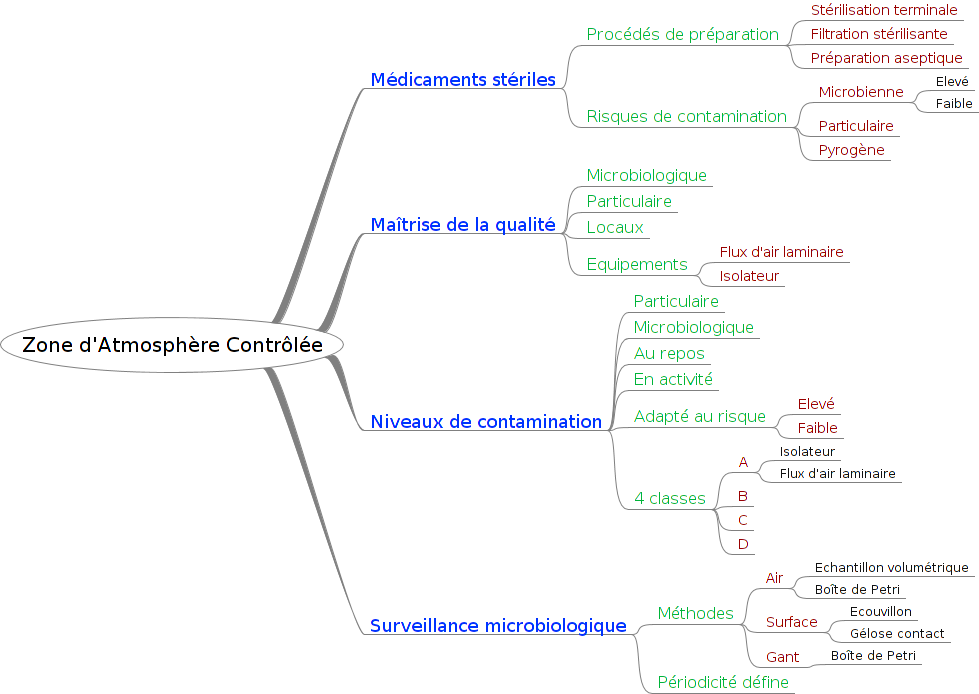
\includegraphics[scale=0.4]{zac.png}
\end{figure}

Aux fins de préparation de médicaments stériles, 4 classes de ZAC sont distinguées. Des recommandations pour la surveillance microbiologique des ZAC sont présentées dans la table \ref{zac}. Les méthodes d'échantillonnages utilisent des boîtes de Petri, des échantillons volumétriques d'air et des contrôles de surface (prélevés au moyen de géloses de contact et/ou écouvillons).
\begin{table}[h]
\caption{Recommandations pour la surveillance microbiologique des zones d'atmosphère controlée en activité. Limites de contamination en unité formant colonie (ufc).\label{zac}}
\begin{center}
\begin{tabular}{|c|c|c|c|c|}
	\hline
	\textbf{Classe} & \textbf{Air} &\textbf{Surfaces} & \textbf{Gants}\\
	\hline
	A & <1 & <1 & <1\\
	B & 10 & 5 & 5\\
	C & 50 & 25 & -\\
	D & 100 & 50 & -\\
	
	\hline
\end{tabular}
\end{center}
\end{table}

La pharmacie de notre établissement prépare des mélanges de nutrition parentérale pour la réanimation néonatale. L'unité de préparation des mélanges de nutrition parentérale de notre établissement est constituée d'un isolateur en classe A dans une zone de préparation en classe D. Afin de surveiller la conformité de notre unité aux exigences des BPP, des prélèvements microbiologiques sont effectués quotidiennement. Une quarantaine de points de prélèvements ont été définis :
\begin{itemize}
 \item Selon le lieu : isolateur ou salle;
 \item Selon le type de prélèvement : air, surface, gant;
 \item Selon le dispositif utilisé : boîte de Petri, gélose contact, écouvillon;
 \item Selon le point précis de prélèvement : gants, champs stériles, balance, automate de fabrication, etc.
 \end{itemize}
Moins d'une dizaine de points sont prélevés quotidiennement. Afin de prélever tous les points chaque semaine, un planning de prélèvement répartit les points à prélever sur l'ensemble de la semaine.

Les prélèvements microbiologiques sont traités par le laboratoire d'hygiène du service de Biologie. En cas de contamination microbiologique de l'isolateur, les résultats (en nombre de colonies) sont communiqués immédiatement par téléphone au pharmacien. L'identification des germes est faite ultérieurement. Dès l'identification des germes, un compte rendu signé par un biologiste est rendu à la pharmacie.

Actuellement les prélèvements effectués et leurs résultats sont enregistrés sur un tableur.
\section{Objectif}
L'objectif de ce projet est de mettre à disposition des utilisateurs un serveur web couplé à système de gestion de base de données qui doit permettre de saisir et consulter les prélèvements microbiologiques et leurs résultats.
\section{Materiel et méthode}

\subsection{Système de gestion de base de données}
 \subsubsection{Base de données postgreSQL}

La base de données postgreSQL (version 9.3) est installée sur le système d'exploitation GNU/Linux (Linux Mint 17.3).
La base de données est nommée \emph{bacterio\_upnp}.


\subsubsection{Création des tables}
\begin{description}
\item[Table disp\_prelev] (Table \ref{disp}) référence les dispositifs de prélèvement. Elle a été créée avec la requête :
\begin{tabbing}
CREATE TABLE disp\_prelev(\\
id SERIAL PRIMARY KEY,\\
disp VARCHAR(50) NOT NULL\\
);
\end{tabbing}
\begin{table}
\caption{Table disp\_prelev \label{disp}}
\begin{center}
\begin{tabular}{|c|c|c|c|}
	\hline
	\textbf{Nom de variable} & \textbf{Type} & \textbf{Clé primaire} & \textbf{Clé étrangère}\\
	\hline
	id & SERIAL & oui &\\
	disp & VARCHAR(50)& &\\
	\hline
\end{tabular}
\end{center}
\end{table}

\item[Table limites\_classes] (Table \ref{classes}) liste les classes microbiologiques, les types de prélèvements et les limites microbiologiques. Elle a été créée avec la requête :
\begin{tabbing}
CREATE TABLE limites\_classes(\\
id SERIAL PRIMARY KEY,\\
classe VARCHAR(10) NOT NULL\\
type VARCHAR(50) NOT NULL\\
limite INTEGER NOT NULL\\
);
\end{tabbing}
\begin{table}
\caption{Table limites\_classes \label{classes}}
\begin{center}
\begin{tabular}{|c|c|c|c|}
	\hline
	\textbf{Nom de variable} & \textbf{Type} & \textbf{Clé primaire} & \textbf{Clé étrangère}\\
	\hline
	id & SERIAL & oui &\\
	classe & VARCHAR(10)& &\\
	type & VARCHAR(50)& &\\
	limite & INTEGER & &\\
	\hline
\end{tabular}
\end{center}
\end{table}

\item[Table points\_prelev] (Table \ref{points}) liste les points de prélèvements utilisés. Elle a été créée avec la requête :
\begin{tabbing}
CREATE TABLE points\_prelev(\\
id SERIAL PRIMARY KEY,\\
point VARCHAR(10) NOT NULL,\\
id\_disp INTEGER NOT NULL REFERENCES disp\_prelev(id)\\
id\_class INTEGER NOT NULL REFERENCES limites\_classes(id),\\
);
\end{tabbing}
\begin{table}
\caption{Table points\_prelev \label{points}}
\begin{center}
\begin{tabular}{|c|c|c|c|}
	\hline
	\textbf{Nom de variable} & \textbf{Type} & \textbf{Clé primaire} & \textbf{Clé étrangère}\\
	\hline
	id & SERIAL & oui &\\
	point & VARCHAR(10)& &\\
	id\_disp & INTEGER & & disp\_prelev(id)\\
	id\_class & INTEGER & & limites\_classes(id)\\
	\hline
\end{tabular}
\end{center}
\end{table}

\item[Table jours\_prelev] (Table \ref{jours}) liste les jours de prélèvements. Elle a été créée avec la requête :
\begin{tabbing}
CREATE TABLE jours\_prelev(\\
id SERIAL PRIMARY KEY,\\
jour VARCHAR(10) NOT NULL,\\
);
\end{tabbing}
\begin{table}
\caption{Table jours\_prelev \label{jours}}
\begin{center}
\begin{tabular}{|c|c|c|c|}
	\hline
	\textbf{Nom de variable} & \textbf{Type} & \textbf{Clé primaire} & \textbf{Clé étrangère}\\
	\hline
	id & SERIAL & oui &\\
	jours & VARCHAR(10)& &\\
	\hline
\end{tabular}
\end{center}
\end{table}


\item[Table planning\_prelev] (Table \ref{planning}) associe des jours de prélèvements et des points de prélèvements. Elle a été créée avec la requête :
\begin{tabbing}
CREATE TABLE planning\_prelev(\\
id\_jour INTEGER NOT NULL REFERENCES jours\_prelev(id),\\
id\_point INTEGER NOT NULL REFERENCES points\_prelev(id),\\
PRIMARY KEY (id\_jour, id\_point)
);
\end{tabbing}
\begin{table}
\caption{Table planning\_prelev \label{planning}}
\begin{center}
\begin{tabular}{|c|c|c|c|}
	\hline
	\textbf{Nom de variable} & \textbf{Type} & \textbf{Clé primaire} & \textbf{Clé étrangère}\\
	\hline
	id\_jour & INTEGER & oui & jours\_prelev(id)\\
	id\_point & INTEGER & oui & points\_prelev(id)\\
	\hline
\end{tabular}
\end{center}
\end{table}

\item[Table prelevements] (Table \ref{prelevements}) liste les prélèvements réalisés. Elle a été créée avec la requête :
\begin{tabbing}
CREATE TABLE prelevements(\\
id SERIAL PRIMARY KEY,\\
date\_prelev DATE NOT NULL,\\
id\_point INTEGER NOT NULL REFERENCES points\_prelev(id)
);
\end{tabbing}
\begin{table}
\caption{Table prelevements \label{prelevements}}
\begin{center}
\begin{tabular}{|c|c|c|c|}
	\hline
	\textbf{Nom de variable} & \textbf{Type} & \textbf{Clé primaire} & \textbf{Clé étrangère}\\
	\hline
	id & SERIAL & oui & \\
	date\_prelev & DATE & &\\
	id\_point & INTEGER & & points\_prelev(id)\\
	\hline
\end{tabular}
\end{center}
\end{table}
\newpage
\item[Table resultats] (Table \ref{resultats}) pour enregistrer les résultats des prélèvements. Elle a été créée avec la requête :

\begin{tabbing}
CREATE TABLE resultats(\\
id SERIAL PRIMARY KEY,\\
id\_prelev INTEGER REFERENCES prelevements(id),\\
\nopagebreak
ufc INTEGER NOT NULL,\\
germe VARCHAR(100),\\
type\_rendu VARCHAR(10) NOT NULL
);
\end{tabbing}
\begin{table}
\caption{Table resultats \label{resultats}}
\begin{center}
\begin{tabular}{|c|c|c|c|}
	\hline
	\textbf{Nom de variable} & \textbf{Type} & \textbf{Clé primaire} & \textbf{Clé étrangère}\\
	\hline
	id & SERIAL & oui & \\
	date\_prelev & DATE & &\\
	id\_point & INTEGER & & points\_prelev(id)\\
	\hline
\end{tabular}
\end{center}
\end{table}

\end{description}

\subsubsection{Peuplement des tables}
Les enregistrements des tables ont été renseignés par des commandes SQL \emph{INSERT}, sauf pour les tables \emph{prelevements} et \emph{resultats}. Ces deux tables ont été renseignées par l'importation de fichiers .csv contenant les données déjà enregistrées sur tableur.
\subsection{Serveur Web}
Le serveur web Apache (version 2.4.7) et installé sur le système d'exploitation GNU/Linux (Linux Mint 17.3).
Les pages Web sont écrites en langage HTML et PHP (version 7.2.4-1)
\section{Résultats}
Le dump de la base de données est fourni sous le nom de fichier : \textbf{bacterio\_upnp.sql}. Toutes les requêtes sont faites avec l'utilisateur \emph{pharmacien} et le mot de passe \emph{zac}.

Le schéma relationnel de la base \emph{bacterio\_upnp} (figure \ref{erd}) a été obtenu par DBVizualizer.
\begin{figure}
\caption{\label{erd}Schéma relationnel de bacterio\_upnp}
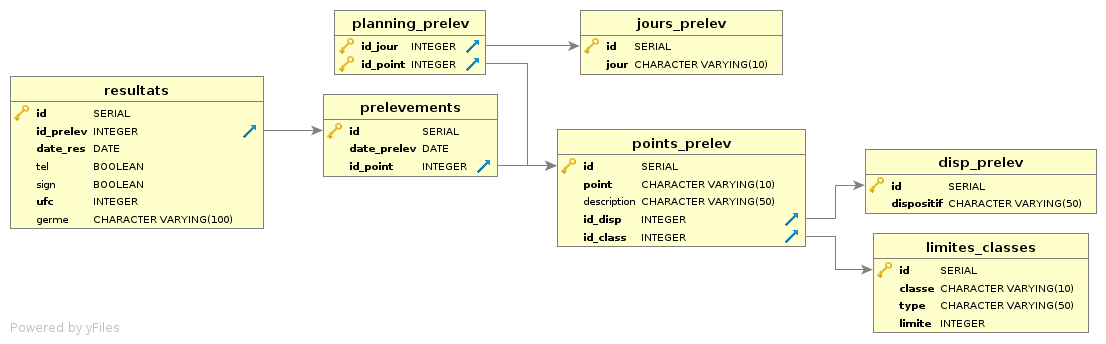
\includegraphics[scale=0.4]{erd.png}
\end{figure}

Les fichiers .php et .html du site web sont les suivants :
\begin{description}
\item[accueil.html :] Présentation de la base de données et accès aux différentes pages par des liens hypertexte.

\end{description}

\section{Discussion}
Discussion
\section{Conclusion}
conclusion





\end{document}
